
\section{The \app Framework Overview}

\begin{figure*}[tbp] \centering
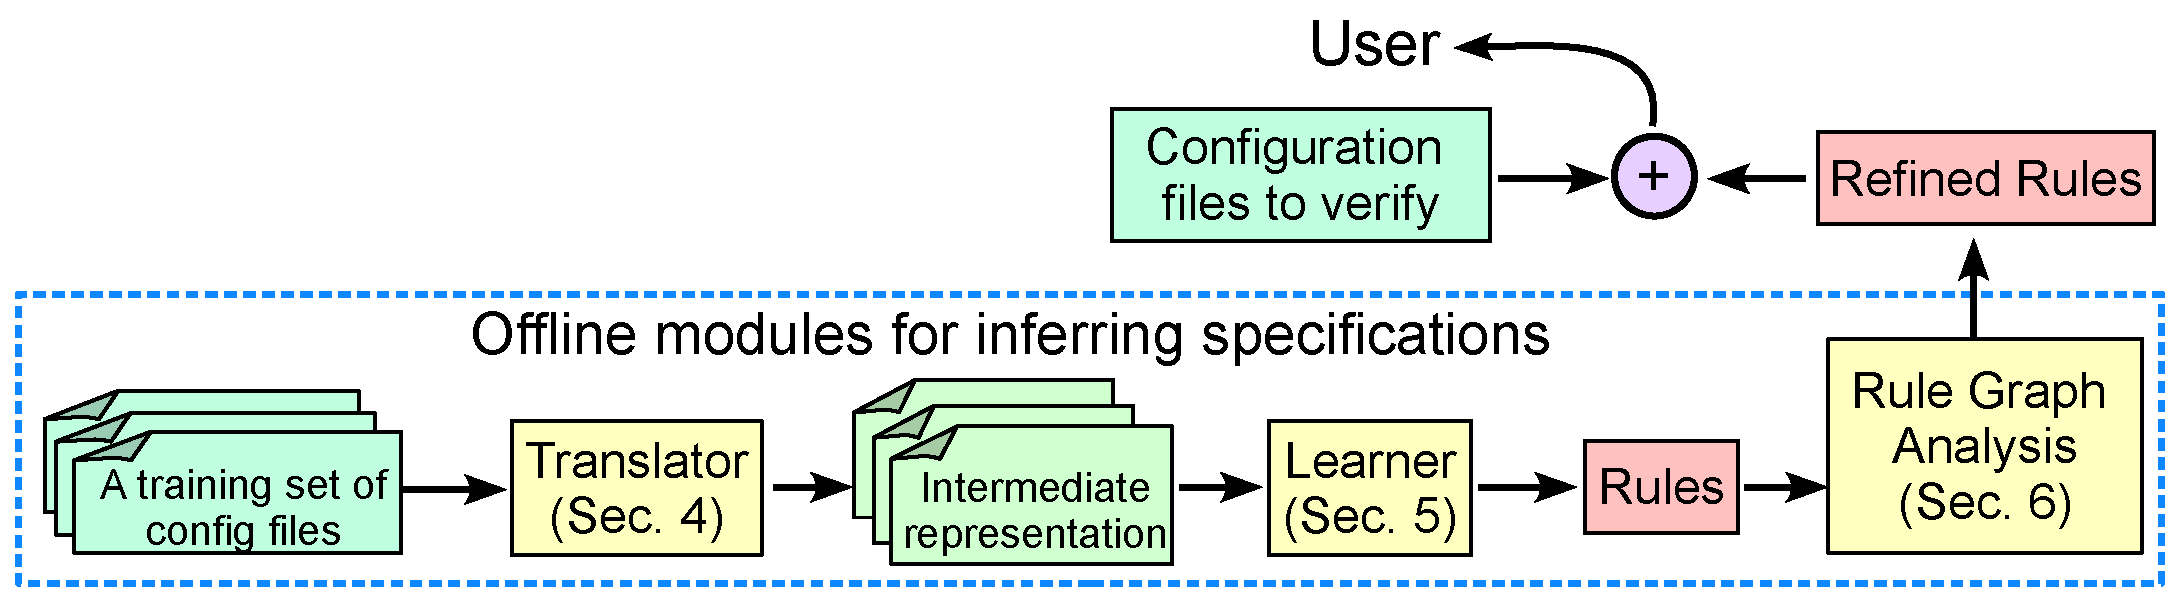
\includegraphics[width=0.99\textwidth]{figs/overview}
\caption{\app's workflow.
  The dashed box is the specification learning module. 
  The yellow components are key modules of \app.}
\label{fig-overview}
\end{figure*}

Figure~\ref{fig-overview} gives an overview of the \app framework.
The main part is dedicated to 
learning and inferring the specification for configuration 
files. This process is done offline, before the user even starts 
to use \app. There are three main steps in the process:
translation, learning, and rule refinement.

\para{Translator}
The translator module first parses the input training  
set of configuration files and transforms them into 
a typed intermediate representation.
Entries in a configuration file follow a key-value pattern, 
where some environmental variable (``key'') is assigned a value.
However, it is not always possible to fully determine the type of the key
by inspecting the value at a single entry~\cite{xu15hey}.
We address this problem 
by introducing {\em probabilistic types}.
Rather than giving a variable a single type, 
we assign several types over a probability distribution that can later be resolved to type upon which we will learn rules.

\para{Learning}
The learner converts the intermediate representation from the translator to a set of rules.
It employs variation on the {\em association rule 
algorithm}~\cite{agrawal1993mining}, to generate this list of rules, which describe properties of a correct configuration file. 
This is a probabilistic verification approach that learns a specification for a correct file over an unlabeled training set of both correct and incorrect configurations files.
The learning algorithm uses various instances of a rule interface to learn different classes of rules, such as ordering or integer relations.
These rules are then considered to be required for any configuration files to be correct, and can be used for verification.

\para{Rule Graph Analysis}
Finally, the logically structured representation of learned rules allows for a further \textit{rule graph analysis}.
The purpose of this module is to refine the learned rules.
To this end, we introduce the concept of a rule graph that can be built from the output of the modified association rule learning algorithm.
We analyze the properties of this graph to construct a ranking of rules by their importance, 
  as well as to produce a measure of complexity for any configuration of the target system.
While the metrics in used in \app are effective, they are not intended to be exhaustive.
The information contained in the structured representation of the learned rules, 
  is a unique benefit of the learning algorithm, that has potential to be leveraged in many new ways.

